
\tikzsetnextfilename{images/refillModelDom_pdf}
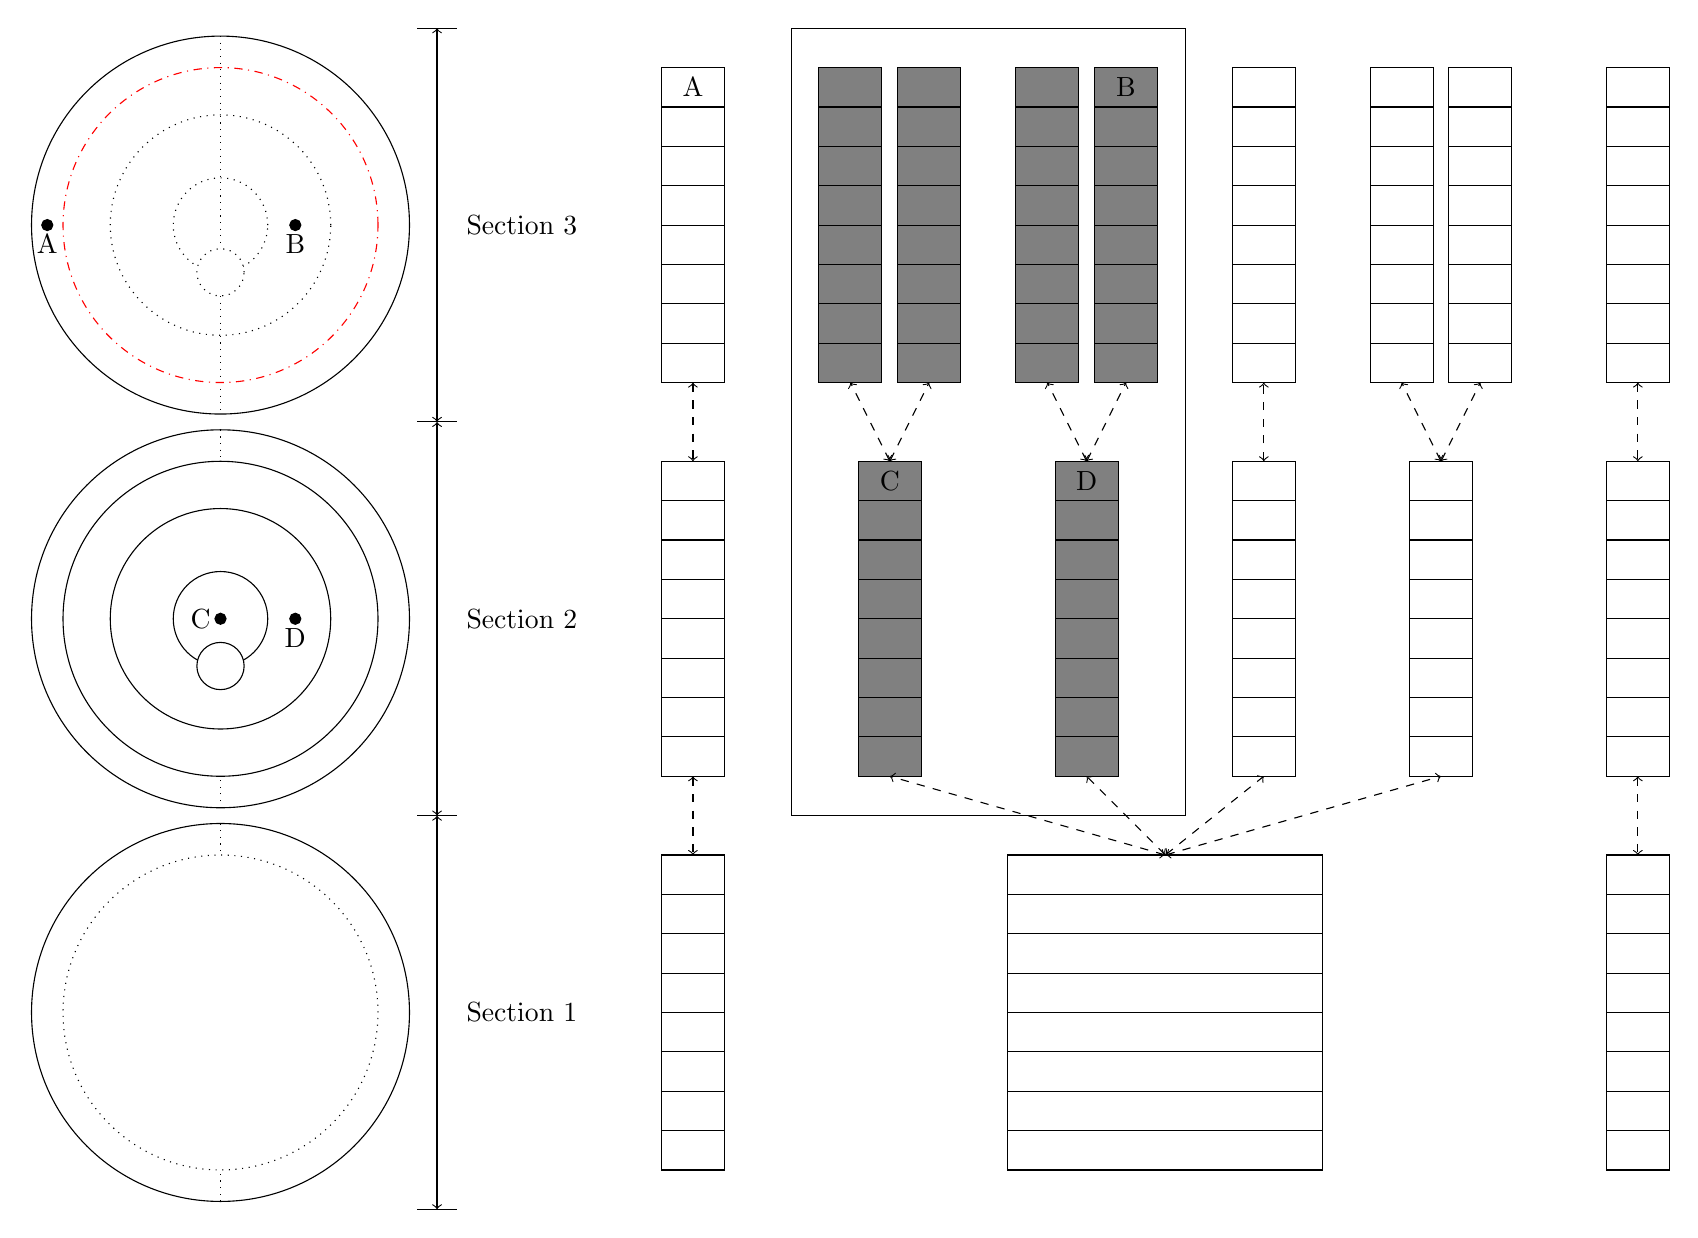
\begin{tikzpicture}

%CIRCLES
%Section 3 Flow Pattern
\draw [dotted] (0.0, 11.9) -- (0, 9.2);
\draw [dotted] (0.0, 8.6) -- (0, 7.1);
\draw [dotted] (0.0, 9.5) circle (0.6);
\draw [dotted] (0.0, 9.5) circle (1.4);
\draw [dashdotted, color=red]  (0.0, 9.5) circle (2.0);
\draw [solid]  (0.0, 9.5) circle (2.4);
\filldraw [dotted, fill=white, draw=black] (0.0, 8.9) circle (0.3);
\filldraw [black] ( 0.95, 9.5) circle (2pt) node[anchor=north]{B};
\filldraw [black] (-2.20, 9.5) circle (2pt) node[anchor=north]{A};	

%Section 2 Flow Pattern
\draw [solid] (0.0, 4.5) circle (0.6);
\draw [solid] (0.0, 4.5) circle (1.4);
\draw [solid] (0.0, 4.5) circle (2.0);
\draw [solid] (0.0, 4.5) circle (2.4);
\filldraw [fill=white, draw=black] (0.0, 3.9) circle (0.3);
\draw [dotted] (0.0, 6.9) -- (0.0, 6.5);
\draw [dotted] (0.0, 2.1) -- (0.0, 2.5);
\filldraw [black] (0.0, 4.5) circle (2pt) node[anchor=east]{C};	
\filldraw [black] ( 0.95, 4.5) circle (2pt) node[anchor=north]{D};

%Section 1 Flow Pattern
\draw [solid]  (0.0, -0.5) circle (2.4);
\draw [dotted] (0.0, -0.5) circle (2.0);
\draw [dotted] (0.0,  1.9) -- (0.0,  1.5);
\draw [dotted] (0.0, -2.9) -- (0.0, -2.5);

%Arrows & Labels
\draw (2.5,12) -- (3,12);
\draw [<->] (2.75,12) -- (2.75,7);
\draw (2.5,7) -- (3,7);
\draw [<->] (2.75,7) -- (2.75,2);
\draw (2.5,2) -- (3,2);
\draw [<->] (2.75,2) -- (2.75,-3);
\draw (2.5,-3) -- (3,-3);
\foreach \y/\ytext in {-0.5/Section 1,4.5/Section 2,9.5/Section 3}
	\draw (3,\y) node [anchor=west] {\ytext};

%RECTANGLES
% Section 3
\foreach \x in {6,18}
{
\draw (\x,9.5) +(-.4,-2) rectangle ++(.4,2);
}

\foreach \x in {8.0, 9.0, 10.5, 11.5}
{
\filldraw [gray] (\x, 9.5) +(-.4,-2) rectangle ++(.4,2);
}

\foreach \x in {6,8,9,10.5,11.5,13.25,15,16,18}
{
\draw (\x,9.5) +(-.4,-2) rectangle ++(.4,2);
}

% Section 2
\foreach \x in {6,18}
{
\draw (\x,4.5) +(-.4,-2) rectangle ++(.4,2);
}

\foreach \x in {8.5, 11}
{
\filldraw [gray] (\x, 4.5) +(-0.4, -2.0) rectangle ++(0.4, 2.0);
}

\foreach \x in {6,8.5,11,13.25,15.5,18}
{
\draw (\x,4.5) +(-.4,-2) rectangle ++(.4,2);
}

% Section 1
\draw (10,-2.5) rectangle (14,1.5);
\draw [black] (10,-2.5) rectangle (14,1.5);
\foreach \x in {6,18}
{
\draw (\x,-0.5) +(-.4,-2) rectangle ++(.4,2);
\draw [black] (\x,-0.5) +(-.4,-2) rectangle ++(.4,2);
}

%Horizontal Partitions
%Section 3
\foreach \x in {6,8,9,10.5,11.5,13.25,15,16,18}
\foreach \y in {8,8.5,...,11.5}
{
\draw (\x,\y) +(-.4,0) -- ++(.4,0);
}
%Section 2
\foreach \x in {6,8.5,11,13.25,15.5,18}
\foreach \y in {3,3.5,...,6.5}
{
\draw (\x,\y) +(-.4,0) -- ++(.4,0);
}

\foreach \x in {7.25,12.25}
{
\draw (\x, 12.0) -- (\x, 2.0);
}

\draw (7.25, 2.0) -- (12.25, 2.0);
\draw (7.25, 12.0) -- (12.25, 12.0);


%Section 1
\foreach \x in {6,18}
\foreach \y in {-2,-1.5,...,1.5}
{
\draw (\x,\y) +(-.4,0) -- ++(.4,0);
}
\foreach \y in {-2,-1.5,...,1.5}
{
\draw (10,\y)--(14,\y);
}

%Flow Lines
\foreach \x in {6,18}
\foreach \y in {2,7}
{
\draw [dashed,<->](\x,\y) +(0,0.5) -- ++(0,-0.5);
}
\foreach \x in {8.5,11,13.25,15.5}
{
\draw [dashed,<->](12,1.5) -- (\x,2.5);
}
\foreach \x in {8,9}
{
\draw [dashed,<->](8.5,6.5) -- (\x,7.5);
}
\foreach \x in {10.5,11.5}
{
\draw [dashed,<->](11,6.5) -- (\x,7.5);
}
\draw [dashed,<->](13.25,6.5) -- (13.25,7.5);
\foreach \x in {15,16}
{
\draw [dashed,<->](15.5,6.5) -- (\x,7.5);
}

%Labels
\draw (6,11.25) node {A};
\draw (11.5,11.25) node {B};
\draw (8.5,6.25) node {C};
\draw (11,6.25) node {D};

\end{tikzpicture}